\begin{minipage}[t]{180mm}
\fcolorbox{black}{white}{
\begin{minipage}[b]{30mm}

\includegraphics[width=0.5\linewidth]{unflogo.pdf}
\end{minipage}
\begin{minipage}[b]{100mm}
\Huge \textbf{UNF NEWZ} \\
\Large -- Stadig uden nok søvn!
\end{minipage}
\begin{minipage}[b]{50mm}
\Large Fredag 19.07.2016 \\
\normalsize Redigeret i \LaTeX\ af \\ SOM, MGS
\end{minipage}
}
\end{minipage}



\begin{minipage}[b]{0.95\linewidth}
\begin{minipage}[t]{0.47\textwidth}
\vspace{1mm}
\section*{Dagens norske haikudikt}
\begin{center}
Sørlandssommer \\
smak av markjordbær \\
bak tynne blusser. \\
\emph{Geir Wigdel}
\end{center}
 

\section*{Ikke-kommutativ studenterrådgiv.}
\emph{Kære brevkasse}


\emph{Hilsen, en trold fra fysik}

\subsection*{Spørgsmål}


{\flushright\emph{Hilsen den ikke-kommutative studenterrådgivning}}

\end{minipage}%
\hfill\begin{minipage}[t]{0.47\textwidth}
\vspace{2mm}
\section*{Vejrudsigt}
\textbf{IMF, AU (fra DMI)}: Temperaturer fra 16 til 23 grader og skyet omkring middag med svag vind fra nordvest. Der forventes et moderat antal græspollen, og et lavt antal bynkepollen.

\textbf{Hogwarts}: Høj sandsynlighed for stjerneskud, og mange ugler på himlen, men der er set dementorer i skoven.

\section*{Fakta om Jylland}
Jylland er en halvø: den anden halvdel er immigreret til Mars, fordi de kom i krig over noget med en næse

\section*{Dagens matematiker}
Hvis du møder en matematiker, så sig noget sødt til hende/ham.

\section*{Dagens sandsynlighed}
Sandsynligheden for at der blandt $51$ er mindst $12$ elever der fordeles til ét kollegie er $1$. 

\end{minipage}

\begin{center}
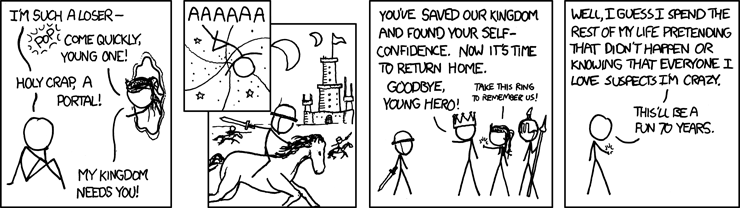
\includegraphics[width=\linewidth]{childrens_fantasy.png}
\tiny Randall Munroe, http://xkcd.com/693/, CC-BY-SA-2.5

\tiny UNF Newz er avisen hvor at ansvarshavende redaktør fralægger sig ethvert ansvar for eventuel plagiering, kaniner, tysk, stavefelj, kaffe, dårlig humor, glemsomhed, katte, store sigmaer, pile, skyer, dårlige oversættelser og alt hvad eventuelle homo sapiens sapiens kunne finde på at holde imod UNF Newz! Dog tager UNF Newz fuld credit og copyright for alle guldkorn, magickort, mus, \TeX, humor, smil, Mortener, kaffe, før-fremtid, ringe og/eller Rubiksterning.
\end{center}
\end{minipage}

